\documentclass[../BTL.tex]{subfiles}
\begin{document}
\section*{Quy định chung}
Dưới đây là một số quy định và hướng dẫn viết BTL mà bắt buộc sinh viên phải đọc kỹ và tuân thủ nghiêm ngặt.

Sinh viên cần đảm bảo tính thống nhất toàn báo cáo (font chữ, căn dòng hai bên, hình ảnh, bảng, margin trang, đánh số trang, v.v.). Để làm được như vậy, sinh viên chỉ cần sử dụng các định dạng theo đúng template BTL này. Khi paste nội dung văn bản từ tài liệu khác của mình, sinh viên cần chọn kiểu Copy là “Text Only” để định dạng văn bản của template không bị phá vỡ/vi phạm.

Tuyệt đối cấm sinh viên đạo văn. Sinh viên cần ghi rõ nguồn cho tất cả những gì không tự mình viết/vẽ lên, bao gồm các câu trích dẫn, các hình ảnh, bảng biểu, v.v. Khi bị phát hiện, sinh viên sẽ không được phép bảo vệ BTL.

Tất cả các hình vẽ, bảng biểu, công thức, và tài liệu tham khảo trong BTL nhất thiết phải được SV giải thích và tham chiếu tới ít nhất một lần. Không chấp nhận các trường hợp sinh viên đưa ra hình ảnh, bảng biểu tùy hứng và không có lời mô tả/giải thích nào.

Sinh viên tuyệt đối không trình bày BTL theo kiểu viết ý hoặc gạch đầu dòng. BTL không phải là một slide thuyết trình; khi người đọc không hiểu sẽ không có ai giải thích hộ. Sinh viên cần viết thành các đoạn văn và phân tích, diễn giải đầy đủ, rõ ràng. Câu văn cần đúng ngữ pháp, đầy đủ chủ ngữ, vị ngữ và các thành phần câu.
Khi thực sự cần liệt kê, sinh viên nên liệt kê theo phong cách khoa học với các ký tự La Mã. Ví dụ, nhiều sinh viên luôn cảm thấy hối hận vì (i) chưa cố gắng hết mình, (ii) chưa sắp xếp thời gian học/chơi một cách hợp lý, (iii) chưa tìm được người yêu để chia sẻ quãng đời sinh viên vất vả, và (iv) viết BTL một cách cẩu thả.

Trong một số trường hợp nhất thiết phải dùng các bullet để liệt kê, sinh viên cần thống nhất Style cho toàn bộ các bullet các cấp mà mình sử dụng đến trong báo cáo. Nếu dùng bullet cấp 1 là hình tròn đen, toàn bộ báo cáo cần thống nhất cách dùng như vậy; ví dụ như sau:

\begin{itemize}
\item Đây là mục 1 – Thực sự không còn cách nào khác tôi mới dùng đến việc bullet trong báo cáo.
\item Đây là mục 2 – Nghĩ lại thì tôi có thể không cần dùng bullet cũng được. Nên tôi sẽ xóa bullet và tổ chức lại hai mục này trong báo cáo của mình cho khoa học hơn. Tôi muốn thầy cô và người đọc cảm nhận được tâm huyết của tôi trong từng trang báo cáo BTL.
\end{itemize}


\section{Đánh dấu (bullet) và đánh số (numering)}
Việc sử dụng danh sách trong LaTeX khá đơn giản và không yêu cầu sinh viên phải thêm bất kỳ gói bổ sung nào. LaTeX cung cấp hai môi trường liệt kê đó là:
\begin{itemize}
\item Đánh dấu (bullet) là kiểu liệt kê không có thứ tự. Để sử dụng kiểu liệt kê đánh dấu, chúng ta khai báo như sau\\ 
\verb$\begin{itemize}$\\
 \verb$\item$ Nội dung thứ nhất được viết ở đây.\\
\verb$\item$ Nội dung thứ hai được viết ở đây.\\
 \verb$\item$ ...\\
\verb$\end{itemize}$
\item Đánh số (numering) là kiểu liệt kê có thứ tự. Để sử dụng kiểu liệt kê đánh số, chúng ta khai báo như sau\\
\verb$\begin{enumerate}$\\
 \verb$\item$ Nội dung thứ nhất được viết ở đây.\\
\verb$\item$ Nội dung thứ hai được viết ở đây.\\
 \verb$\item$ ...\\
\verb$\end{enumerate}$
\end{itemize}
Chú ý các nội dung trình bày trong cả hai môi trường liệt kê theo sau lệnh \verb$\item$. Ngoài ra LaTeX còn cung cấp một số kiểu liệt kê khác, sinh viên có thể tham khảo tại \url{https://www.overleaf.com/learn/latex/Lists}
\section{Cách thêm bảng}
\begin{table}[h!]
\centering
\begin{tabular}{||c c c c||} 
 \hline
 Col1 & Col2 & Col2 & Col3 \\ [0.5ex] 
 \hline\hline
 1 & 6 & 87837 & 787 \\ 
 2 & 7 & 78 & 5415 \\
 3 & 545 & 778 & 7507 \\
 4 & 545 & 18744 & 7560 \\
 5 & 88 & 788 & 6344 \\ [1ex] 
 \hline
\end{tabular}
\caption{Table to test captions and labels.}
\label{table:1}
\end{table}
Bảng \ref{table:1} là ví dụ về cách tạo bảng. Tất cả các bảng biểu phải được đề cập đến trong phần nội dung và phải được phân tích và bình luận.  Chú ý: Tạo bảng trong Latex khá phức tạp và mất thời gian, vì vậy sinh viên có thể sử dụng các công cụ hỗ trợ tạo bảng (Ví dụ: \url{https://www.tablesgenerator.com/}).
Sinh viên có thể tìm hiểu sâu hơn về cách chèn ảnh trong Latex tại link \url{https://www.overleaf.com/learn/latex/Tables}.

\section{Chèn hình ảnh}
\begin{figure}
\centering
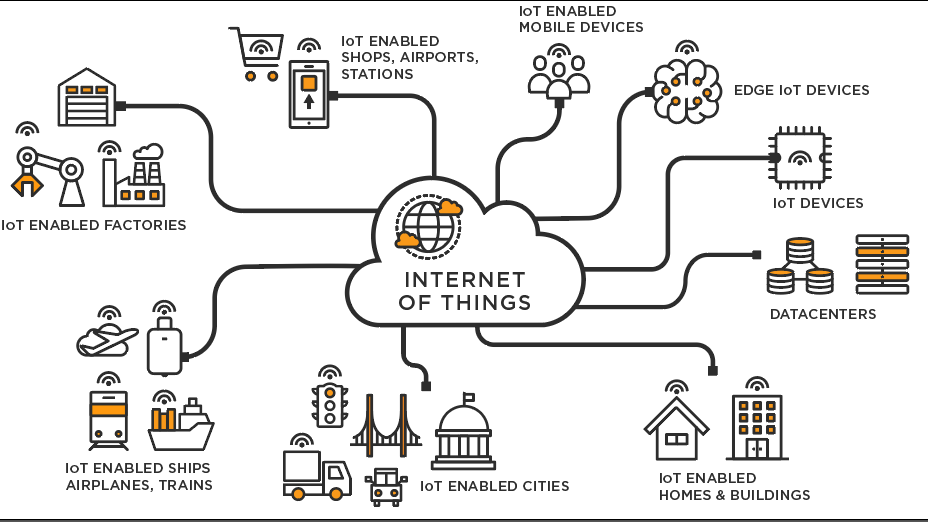
\includegraphics[width=0.75\linewidth]{Hinhve/IoT.png}
\caption{Internet vạn vật}
\label{fig:iot}
\end{figure}

Hình \ref{fig:iot} là ví dụ về cách chèn ảnh. Lưu ý chú thích của hình vẽ được đặt ngay dưới hình vẽ. Sinh viên có thể tìm hiểu sâu hơn về cách chèn ảnh trong Latex tại \url{https://www.overleaf.com/learn/latex/Inserting_Images}.

Chú ý, tất cả các hình vẽ phải được đề cập đến trong phần nội dung và phải được phân tích và bình luận. 

\section{Tài liệu tham khảo}
\paragraph{Cách liệt kê}\mbox{}

Áp dụng cách liệt kê theo quy định của IEEE. Ví dụ của việc trích dẫn như sau \cite{scott2013sdn}. Cụ thể, sinh viên sử dụng lệnh \verb!\cite{}! như sau \cite{ashton2009internet}. Chỉ những tài liệu được trích dẫn thì mới xuất hiện trong phần Tài liệu tham khảo. Tài liệu tham khảo cần có nguồn gốc rõ ràng và phải từ nguồn đáng tin cậy. Hạn chế trích dẫn tài liệu tham khảo từ các website, từ wikipedia.
\paragraph{Các loại tài liệu tham khảo}\mbox{}

Các nguồn tài liệu tham khảo chính là sách, bài báo trong các tạp chí, bài báo trong các hội nghị khoa học và các tài liệu tham khảo khác trên internet.

\section{Cách viết phương trình và công thức toán học}
Các gói amsmath, amssymb, amsfonts hỗ trợ viết phương trình/công thức toán học đã được bổ sung sẵn ở phần đầu của file main.tex. Một ví dụ về tạo phương trình \eqref{pt31} như sau 
\begin{equation}\label{pt31}
    F(x) = \int^a_b \frac{1}{3}x^3
\end{equation}
Phương trình \ref{pt31} là ví dụ về phương trình tích phân. Một phương trình khác không được đánh số thứ tự (gán nhãn)
\begin{equation*}\label{pt32}
    x[t_n] = \frac{1}{\sqrt{N}} \sum_{k=0}^{N-1}X[f_k]e^{j 2\pi n k/N}
\end{equation*}
Phương trình này thể hiện phép biến đổi Fourier rời rạc ngược (IDFT).



\end{document}